\documentclass[11pt,a4paper]{article}

\usepackage[utf8]{inputenc}
\usepackage[T1]{fontenc}
\usepackage[margin=2.2cm]{geometry}
\usepackage{amsmath,amssymb}
\usepackage{graphicx}
\usepackage{booktabs}
\usepackage{array}
\usepackage{tabularx}
\usepackage[numbers,sort&compress]{natbib}
\usepackage[hidelinks]{hyperref}
\usepackage{setspace}
\usepackage{caption}
\captionsetup{font=small,labelfont=bf}

\setlength{\parskip}{0.4em}
\setlength{\parindent}{0pt}
\setstretch{1.08}
\emergencystretch=2em

\newcommand{\tresp}{t_{\mathrm{resp}}}

\title{\textbf{Decoding Pre-Response EEG Signatures of Choice, Accuracy, and Confidence in Perceptual Decision-Making}}

\author{%
\footnotesize\begin{tabular}{@{\extracolsep{0.8em}}ccc@{}}
 \begin{tabular}[t]{@{}c@{}}Amith Pradhaan\\ Assistant Professor\\ \textit{Dept.\ of Computer Science,}\\ \textit{BMS College of Engineering}\\ Bangalore, India\\ {\footnotesize amithpradhaan.cse@bmsce.ac.in}\end{tabular} &
 \begin{tabular}[t]{@{}c@{}}Pranav Easwar\\ Student\\ \textit{Dept.\ of Computer Science,}\\ \textit{BMS College of Engineering}\\ Bangalore, India\\ {\footnotesize pranaveaswar.cs23@bmsce.ac.in}\end{tabular} &
 \begin{tabular}[t]{@{}c@{}}Manoj Kulkarni\\ Student\\ \textit{Dept.\ of Computer Science,}\\ \textit{BMS College of Engineering}\\ Bangalore, India\\ {\footnotesize manojkulkarni.cs23@bmsce.ac.in}\end{tabular} \\[2.8em]
 \begin{tabular}[t]{@{}c@{}}Padma Deepak\\ Student\\ \textit{Dept.\ of Computer Science,}\\ \textit{BMS College of Engineering}\\ Bangalore, India\\ {\footnotesize padmadeepak.cs23@bmsce.ac.in}\end{tabular} &
 \begin{tabular}[t]{@{}c@{}}Siddhant Sawhney\\ Student\\ \textit{Dept.\ of Computer Science,}\\ \textit{BMS College of Engineering}\\ Bangalore, India\\ {\footnotesize siddhantsawhney.cs23@bmsce.ac.in}\end{tabular} &
\end{tabular}}
\date{}

\begin{document}
\maketitle

\begin{abstract}
\noindent Scalp EEG carries confidence-related information before an explicit response, but it is unclear whether such pre-response activity predicts the upcoming choice, its accuracy, or the calibration of confidence. Using a public simultaneous EEG-fMRI random-dot motion dataset (24 participants, 7,377 trials), we decoded choice, accuracy, and confidence from a 600\,ms window ending 150\,ms before the response, with leave-one-subject-out validation and permutation tests. Held-out-subject AUC was 0.526 for choice, 0.535 for accuracy, and 0.540 for confidence, all above chance. After removing linear dependence on response time, only choice decoding remained significant. High-confidence errors were not separable from low-confidence errors, and decoded neural confidence did not predict next-trial behavior, whereas reported confidence predicted choice repetition. Nonlinear and alternative-feature decoders did not outperform logistic regression. Pre-response EEG therefore carries weak information, largely related to response time.
\end{abstract}

\noindent\textbf{Keywords:} Perceptual decision-making, Electroencephalography, Decision confidence, Single-trial decoding, Overconfidence, Cross-validation

%====================================================================
\section{Introduction}

Whether the electrical activity of the brain contains information about a decision before the decision is expressed is a central question in the neuroscience of perceptual decision-making. Three claims are often conflated. First, EEG activity may be related to (correlate with) a person's choice or confidence. Second, EEG activity may allow the choice, its accuracy, or the reported confidence to be predicted on a single trial ahead of time. Third, EEG activity may cause or determine the choice. Observational EEG can support at most the first two claims; the third requires an interventional manipulation such as brain stimulation and is outside the scope of this study.

The dataset analysed here \cite{r1,r2} already supports the first claim: a stimulus-independent EEG component that discriminates confidence appeared before the explicit choice and confidence report and was consistent with a confidence measure from an accumulation-to-bound model \cite{r2}. Repeating that analysis would add little. We therefore pursue the second claim, prediction, and decompose it into four research questions. \textbf{RQ1 (choice):} can pre-response EEG predict the identity of the upcoming left or right motion judgment? \textbf{RQ2 (accuracy):} can it predict whether that judgment will be correct? \textbf{RQ3 (calibration):} can it distinguish the four joint states of accuracy and confidence, and in particular do high-confidence errors, an operational marker of overconfidence, differ from low-confidence errors? \textbf{RQ4 (sequential effects):} does the neural confidence state on trial $N$ predict behavior on trial $N{+}1$?

Evidence linking EEG to error detection and confidence comes largely from components that follow the response, such as the error positivity \cite{r3,r4}, which cannot be used to predict a decision before it is made. Information available before the response, in a window that excludes the response and its immediate motor preparation, has received less attention, and one study with a different paradigm reported no above-chance pre-response decoding of confidence \cite{r5}. Whether pre-response EEG supports prediction of choice, accuracy, and calibration in a perceptual task therefore remains open.

The distinction matters for how decoding results are interpreted. A signal that is merely correlated with confidence in an average over trials can be useless for single-trial prediction, and a signal that predicts well within a participant may not transfer to a new participant. Prediction claims therefore require out-of-sample evaluation at the level at which generalization is claimed, and, for targets that covary with response speed, a control that shows the prediction does not simply reflect speed.

This paper makes six contributions. (i) We define a leakage-controlled prediction window of fixed length that ends a fixed buffer before each trial's own response. (ii) We decode choice, accuracy, and confidence in 24 participants with leave-one-subject-out validation and permutation inference. (iii) We add an explicit control for response-time information, which accounts for the accuracy and confidence effects. (iv) We compare the primary decoder with five alternative classifiers and three feature sets. (v) We report the full class balance and subject diversity of the rare high-confidence error cell before any calibration analysis. (vi) We fixed the analysis plan before inspecting decoding results and report a sensitivity analysis over the window grid. The results are modest, and we report them as such.

%====================================================================
\section{Related Work}

\subsection{Choice from pre-response EEG}

A centro-parietal positivity (CPP) has been characterized as a domain-general decision variable that builds up to a threshold before a perceptual report \cite{r6}. In a random-dot motion task its build-up rate scaled with evidence strength and predicted reaction time within coherence levels \cite{r7}. Because the CPP indexes the unsigned strength of accumulated evidence \cite{r8}, decoding the side of a left or right choice must also draw on signals that differ between alternatives, including motor preparation; classic motor potentials were shown to reflect the continuing involvement of the motor system in value-based decisions \cite{r9}. Single-trial linear classifiers over EEG components were established by Philiastides et al.\ \cite{r10} and extended by Ratcliff et al.\ \cite{r11}, who showed that single-trial component amplitudes sort response times and choices by the quality of evidence in a diffusion model; a review is given in \cite{r12}. Free-choice paradigms decoded internally generated choices from fMRI seconds before awareness \cite{r13,r14}, but they differ from evidence-driven perceptual discrimination and serve here only as precedent.

\subsection{Pre-response EEG and accuracy}

The same single-trial framework separates correct from incorrect trials: early and late EEG components predicted decision accuracy and were distinct from a component related to task difficulty \cite{r10}. CPP build-up and threshold crossing relate to accuracy and speed \cite{r6,r7}, and single-trial CPP slopes were related to the drift parameter of an accumulator model \cite{r15}.

\subsection{Confidence, calibration, and high-confidence errors}

Boldt and Yeung \cite{r3} showed that the error positivity (Pe) varies in a graded way with confidence independent of accuracy, and that decoders of error detection predict confidence differences among correct trials, suggesting shared mechanisms for error detection and confidence. In masked-digit tasks the error-related negativity (ERN) appeared only for conscious trials, although errors could still be detected above chance without it \cite{r16}, and response accuracy could be decoded only when the target was conscious \cite{r17}. Desender et al.\ \cite{r4} propose that the Pe reflects post-decisional evidence accumulation, whereas Rausch et al.\ \cite{r18} found confidence-related activity both after stimulus onset and after the response and argued that markers of confidence and error awareness are partly distinct. Parietal EEG signals have also been reported to index subjective evidence and, later, a confidence-like quantity \cite{r8}. We use ``overconfidence'' operationally, as a high-confidence error. This is a coarse, single-trial definition compared with measures of metacognitive sensitivity \cite{r19}, and linking attenuated error signals to overconfidence is our interpretation rather than a finding of the studies cited above.

\subsection{Sequential effects}

Choice history biases were explained by the accumulation of confidence-modulated decision variables across trials \cite{r20}, and pupil-linked arousal driven by decision uncertainty increased the tendency to alternate on the next trial \cite{r21}. Desender et al.\ \cite{r22} showed that decision bounds depend on the confidence reported on the previous trial and that a confidence-sensitive centro-parietal EEG component predicted the bound increase; confidence-related EEG decoding has also been linked to information seeking \cite{r5}.

Table~\ref{tab:related} compares the most closely related EEG studies on the dimensions that matter for the present question: which signal was examined, when relative to the stimulus or response, and what was found.

\begin{table}[ht]
\centering
\caption{Closely related EEG studies}
\label{tab:related}
\small
\begin{tabularx}{\textwidth}{@{}l>{\raggedright\arraybackslash}X>{\raggedright\arraybackslash}X@{}}
\toprule
\textbf{Study} & \textbf{Signal and timing} & \textbf{Main finding}\\
\midrule
\cite{r10} & Single-trial components about 170 and 300\,ms after the stimulus & Components predicted accuracy; a separate component tracked difficulty\\
\cite{r2} & Single-trial component before the choice and the confidence report (EEG-fMRI) & Stimulus-independent confidence component, linked to ventromedial prefrontal activity\\
\cite{r3} & Pe after the response & Pe graded with confidence independent of accuracy\\
\cite{r18} & 350--500\,ms after the stimulus and 250--350\,ms after the response & Two confidence-related periods; post-response activity partly distinct\\
\cite{r5} & Time-resolved decoding from the initial decision onward & Confidence decodable; no above-chance decoding before the response\\
\cite{r22} & Centro-parietal component sensitive to confidence & Predicted the bound increase on the next trial\\
\bottomrule
\end{tabularx}
\end{table}

In contrast with this literature, which mostly concerns post-response or stimulus-locked components and within-subject effects, we test out-of-subject prediction from a window that ends before the response, and we control for response time explicitly. Methodologically, small decoding effects in small samples can exceed analytic chance levels by chance \cite{r23}, which is why we rely on permutation inference and report effect sizes together with their null distribution.

%====================================================================
\section{Dataset and Task}

We used the open dataset of Gherman and Philiastides \cite{r1,r2} (OpenNeuro ds002739, CC0 license): 24 participants, two runs each, recorded with simultaneous EEG-fMRI during a speeded left or right random-dot motion discrimination at an individually calibrated coherence (targeting about 75\% accuracy). After the response, participants rated confidence on a 9-point scale whose on-screen orientation was randomized across trials to decorrelate motor preparation from the report. We used the preprocessed EEG supplied with the dataset: scanner-gradient artifacts removed by template subtraction, a 12\,ms median filter, 0.5 to 40\,Hz band-pass filtering, 1000\,Hz sampling, principal-component removal of ocular and ballistocardiogram components, and baseline correction over the 100\,ms before stimulus onset. Per trial we used the stimulus onset, response time (RT), motion direction, choice, accuracy, and confidence rating. Low confidence was defined as ratings 1 to 3 and high confidence as ratings 7 to 9, following the dataset authors' split into the lowest and highest three ratings; ratings 4 to 6 were labeled medium.

A pilot characterization of one run (participant 1, run 1; 158 trials) in our earlier analysis showed only five high-confidence errors, which is too few for single-participant decoding; we reproduced that pilot exactly from the raw files. We therefore pooled all participants and runs and verified that the rare cell is spread across participants (Section~\ref{sec:behavior}).

Each run contained 160 task trials. The dataset authors excluded trials with missing or invalid responses before releasing the event files, and we used only the remaining valid trials, which were also the only ones with EEG epochs in the release. Consecutive trials were identified through the original trial index so that trial pairs in the sequential analysis are truly adjacent even where invalid trials were removed. Motion direction was coded 0 and 180 degrees and the choice 1 (left) or 2 (right); the recorded accuracy agrees with the mapping 0 degrees to right and 180 degrees to left on all 7,377 trials.

%====================================================================
\section{Methods}

\subsection{Epoching and window definition}

Preprocessed EEG was low-pass decimated to 250\,Hz. Because the data were already band-limited to 40\,Hz, this step does not remove information of interest. To avoid contamination by the response, we define for every trial a window of length $L$ that ends a buffer $B$ before that trial's own response time $\tresp$. The mean amplitude of channel $c$ in the window is
\begin{equation}
x_c = \frac{1}{n_w}\sum_{t=t_0}^{t_1-1} e_c(t),
\label{eq:window}
\end{equation}
where $t_0=\tresp-B-L$, $t_1=\tresp-B$, $e_c(t)$ is the EEG of channel $c$, and $n_w$ is the number of samples in the window. A trial is retained only if $\mathrm{RT}\geq L+B$, so that the window lies entirely after stimulus onset. We examined $L$ from 200 to 800\,ms and $B$ from 0 to 350\,ms. The primary window was fixed by a rule that uses trial retention and never decoding performance: among combinations with $B\geq 100$\,ms and at least 80\% pooled retention, choose the largest $L$. This gave $L=600$\,ms and $B=150$\,ms, retaining 6,090 of 7,377 trials (82.6\%; Fig.~\ref{fig:window}). Decoding performance over the grid is reported only as a sensitivity analysis.

\begin{figure}[ht]
\centering
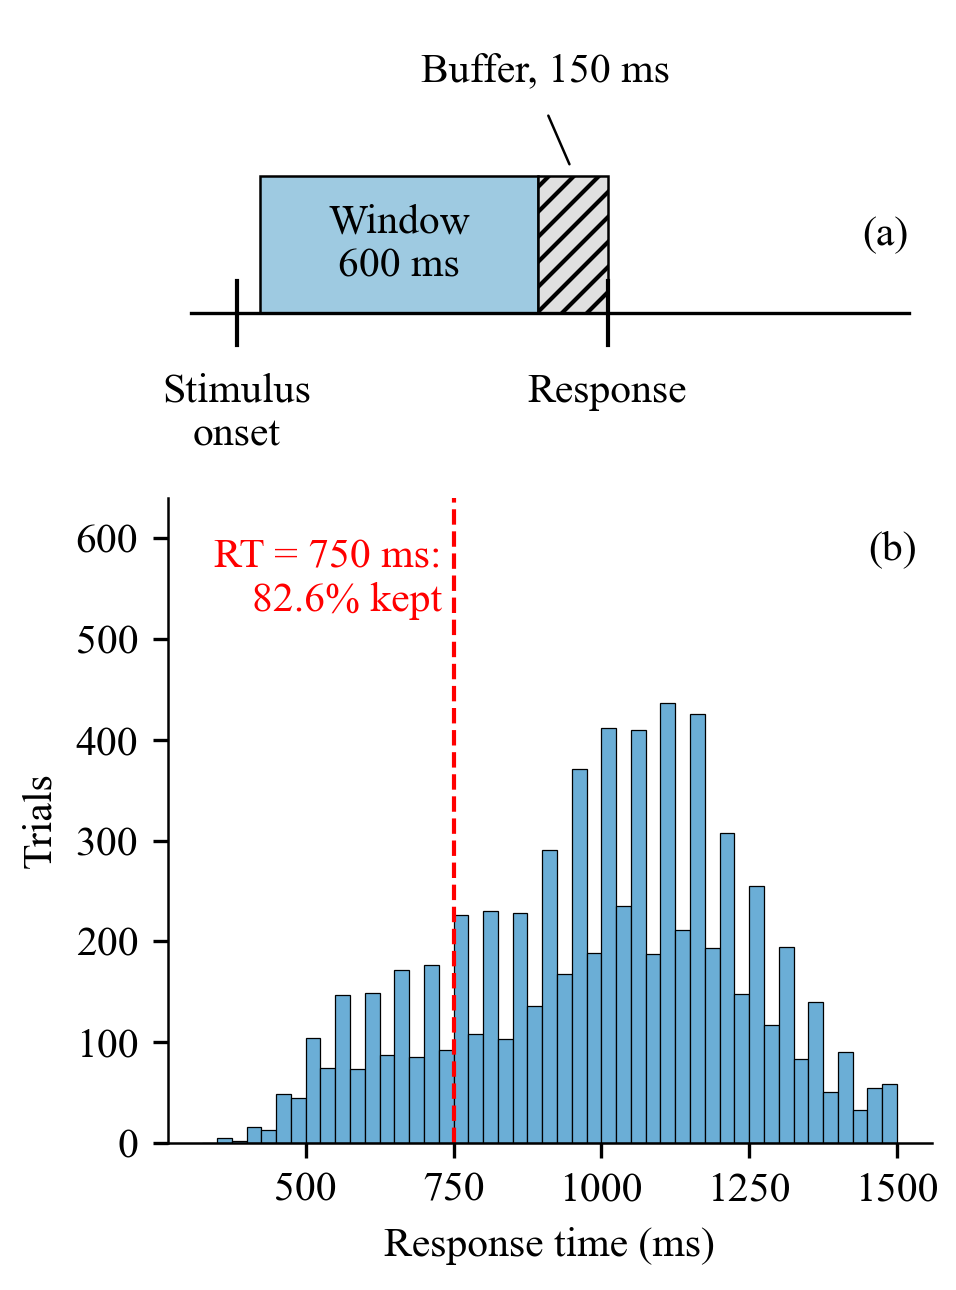
\includegraphics[width=0.5\textwidth]{figures/fig1.png}
\caption{Prediction window. (a) Schematic of the fixed-length window ending a buffer before the response. (b) Distribution of response times for all trials; trials left of the dashed line are too fast for the selected window and are excluded.}
\label{fig:window}
\end{figure}

Eleven of the 64 channels were unavailable in at least one participant after the dataset authors' channel rejection, so all analyses use the 53 channels available in every participant.

\subsection{Single-trial decoder}

We adopt the single-trial spatial-integration linear classifier used for this dataset \cite{r2,r10,r12}: the window-averaged channel vector $\mathbf{x}$ is projected onto a spatial weight vector $\mathbf{w}$ to give one discriminant value per trial,
\begin{equation}
s=\mathbf{w}^{\top}\mathbf{x}+b,
\label{eq:score}
\end{equation}
where $\mathbf{w}$ and $b$ minimize the class-weighted regularized logistic loss
\begin{equation}
\tfrac{1}{2}\lVert\mathbf{w}\rVert^{2}+C\sum_{i}\omega_i\ln\!\bigl(1+\exp(-y_i(\mathbf{w}^{\top}\mathbf{x}_i+b))\bigr)
\label{eq:loss}
\end{equation}
with labels $y_i\in\{-1,+1\}$, class weights $\omega_i$ inversely proportional to class frequency, and $C=0.1$ fixed in advance ($C=0.01$ and $1$ are reported as checks). Features were standardized within each participant using only that participant's own unlabeled data. As a robustness check for the high-dimensional, small-sample regime we also evaluated shrinkage-regularized linear discriminant analysis \cite{r24,r25} and, as a supplement, a spatiotemporal variant with four sub-bin means per channel. All model fitting used training participants only.

\subsection{Comparison decoders}

To test whether the results depend on the primary decoder, we compared it with five alternatives, all evaluated on the same trials, window, and LOSO splits: shrinkage LDA, a linear support vector machine ($C=0.01$), an RBF-kernel support vector machine ($C=1$), a random forest (300 trees, minimum leaf size 20), and a multilayer perceptron (one hidden layer of 32 units, L2 penalty 0.1, early stopping). Besides the window-mean amplitude we used four sub-bin means (spatiotemporal), the log variance of each channel over the window (a power feature), and their concatenation with the mean amplitude. Hyperparameters were fixed in advance in an amendment to the analysis plan, written after the main results were known, and were not tuned, to avoid leakage. Each comparison decoder was also run on RT-residualized features, and its participant AUCs were compared with those of the primary decoder by a paired Wilcoxon signed-rank test with Holm correction within target and feature variant. No permutation test was run for these decoders.

\subsection{Validation and inference}

Because trials from one participant are not independent, the primary scheme is leave-one-subject-out (LOSO) cross-validation. We report the area under the ROC curve,
\begin{equation}
\mathrm{AUC}=P(s_{+}>s_{-})+0.5\,P(s_{+}=s_{-}),
\label{eq:auc}
\end{equation}
where $s_{+}$ and $s_{-}$ are the scores of a randomly drawn trial of the positive and the negative class, for each held-out participant (mean and standard deviation over participants) and for the pooled out-of-subject scores. Chance level was estimated by permutation rather than assumed analytically \cite{r23,r26}: labels were shuffled within participant, the whole LOSO procedure was repeated 500 times, and the one-sided $p$-value is (1 + number of permuted means at least as large as observed)\,/\,501, so the smallest attainable value is 0.002. Within-participant stratified 10-fold cross-validation is reported as a supplement; it replaces the leave-one-trial-out scheme in our earlier plan to make permutation inference computationally feasible.

\subsection{Control for response time}

Accuracy and confidence are related to response time (Section~\ref{sec:behavior}), and a response-locked window is not independent of RT. We therefore (a) decoded each target from log RT alone and (b) repeated every decoding analysis after removing the linear dependence of each feature on log RT within participant,
\begin{equation}
\tilde{\mathbf{x}}=\mathbf{x}-\boldsymbol{\beta}\,z(\ln\mathrm{RT}),
\label{eq:resid}
\end{equation}
where $z(\cdot)$ is the within-participant z-score and $\boldsymbol{\beta}$ is the least-squares coefficient vector. This step uses no outcome labels. It is not part of the original plan; it was added after a four-participant smoke test showed that RT alone predicted confidence well, and before any full-sample result was inspected. As a further check that does not rely on a linear model, we computed the AUC of the main out-of-subject scores within participant-specific RT terciles and averaged over terciles and participants.

\subsection{Time-resolved analysis}

To examine how information evolves toward the response, and to test the rationale for the buffer, we repeated the decoding with 100\,ms windows (step 50\,ms) from 750\,ms to 0\,ms before the response, using trials with RT of at least 750\,ms so that every window lies after stimulus onset. Each window used the same decoder and LOSO scheme, with and without RT residualization. For each window a one-sided one-sample $t$-test of the participant AUCs against 0.5 was computed and Holm-corrected over the 14 windows per target. This analysis is descriptive and was added after the primary analysis.

\subsection{Evaluation protocol}

\begin{table}[ht]
\centering
\caption*{\textbf{Algorithm 1.} Out-of-participant evaluation}
\small
\begin{tabularx}{\textwidth}{@{}X@{}}
\toprule
\textbf{Input:} trials with EEG, RT, labels, participant ID; $L$, $B$, $C$\\
\midrule
1. Keep trials with $\mathrm{RT}\geq L+B$; compute window means (Eq.~\ref{eq:window}).\\
2. Standardize each feature within participant (no labels).\\
3. For each participant $k$: train on all other participants (Eq.~\ref{eq:loss}); score all trials of $k$ (Eq.~\ref{eq:score}).\\
4. Compute AUC per participant (Eq.~\ref{eq:auc}); average over participants.\\
5. Repeat steps 3--4 with labels shuffled within participant, 500 times; obtain the permutation $p$-value.\\
6. Repeat steps 2--5 on RT-residualized features (Eq.~\ref{eq:resid}).\\
\midrule
\textbf{Output:} mean AUC, permutation $p$, RT-controlled AUC\\
\bottomrule
\end{tabularx}
\end{table}

\subsection{Reproducibility and computing}

The raw data are public. The analysis used a laptop with an 8-core processor and 8\,GB of memory, with raw files streamed participant by participant and reduced to 250\,Hz epochs (about 0.7\,GB in total), and ran with Python 3.9, NumPy 1.26, scikit-learn 1.0, and statsmodels 0.13. The window rule, regularization strength, validation scheme, and feasibility threshold for RQ3 were written in an analysis plan before any full-sample decoding result was inspected; the deviations from that plan are the RT control, the time-resolved analysis, the comparison decoders (a second amendment, with fixed hyperparameters), and the replacement of leave-one-trial-out by 10-fold cross-validation, and all are labeled in the text. Permutation seeds are fixed, so all numbers can be regenerated.

\subsection{Calibration analysis (RQ3)}

Accuracy was crossed with the low and high confidence classes, giving four cells: correct/low, correct/high, incorrect/low, and incorrect/high. A four-way analysis was attempted only if the incorrect/high cell contained at least 100 trials from at least 12 participants with no participant contributing more than 20\% (rule fixed in advance). We also evaluated pairwise contrasts (incorrect/high versus incorrect/low, versus correct/high; incorrect/low versus correct/low) with the same LOSO and permutation procedure, and a two-stage analysis in which the out-of-subject accuracy-decoder score is compared between incorrect/high and incorrect/low trials by a within-participant permutation test, with within-participant Spearman correlations between the reported confidence and the score.

\subsection{Sequential analysis (RQ4)}

For consecutive valid trials $N$ and $N{+}1$ in the same run we took as the neural confidence state the out-of-subject high-versus-low-confidence decoder score on trial $N$, applied to all trials and z-scored within participant ($S$), and the z-scored reported confidence ($C$) as a behavioral benchmark. Choice repetition was modeled by a logistic generalized estimating equation (GEE) \cite{r27} with participant clusters and an exchangeable working correlation:
\begin{equation}
\operatorname{logit}P(\mathrm{repeat})=\beta_0+\beta_1 S+\beta_2 D+\beta_3 A+\beta_4 T,
\label{eq:gee}
\end{equation}
where $D$ indicates a repeated motion direction, $A$ is the accuracy on trial $N$, and $T$ is $\ln\mathrm{RT}$ on trial $N$. A supplementary model adds the $D\times A$ interaction. Log RT and accuracy on trial $N{+}1$ were analyzed analogously. The decision bound was not estimated because no diffusion model was fitted; RT and accuracy on trial $N{+}1$ are used as proxies.

%====================================================================
\section{Results}

\subsection{Behavior and class balance}
\label{sec:behavior}

The analysis includes 24 participants, 48 runs, and 7,377 valid trials. Table~\ref{tab:behavior} summarizes the behavior. Accuracy averaged 76.0\% (SD 5.2), close to the calibrated target, and mean RT was 992\,ms. Confidence was higher on correct than on incorrect trials (5.73 versus 4.33), and RT was negatively related to confidence (mean within-participant Spearman $\rho=-0.26$) and to accuracy ($\rho=-0.18$). The selected window retained 6,090 trials. The retained trials are slower, less accurate (74.6\% versus 82.4\%), and less confident (5.21 versus 6.28) than the 1,287 excluded trials, so the decoding results apply to these slower trials.

\begin{table}[ht]
\centering
\caption{Dataset and behavior}
\label{tab:behavior}
\small
\begin{tabular}{@{}ll@{}}
\toprule
\textbf{Measure} & \textbf{Value}\\
\midrule
Participants / runs & 24 / 48\\
Valid trials & 7,377\\
Trials per participant & 290--318\\
Accuracy, mean (SD) & 76.0\% (5.2)\\
RT, mean (SD) & 992 (239) ms\\
Confidence, mean (SD) & 5.39 (2.15)\\
Trials in window & 6,090 (82.6\%)\\
Channels used & 53\\
\bottomrule
\end{tabular}
\end{table}

Table~\ref{tab:cells} gives the joint distribution of accuracy and confidence. The incorrect/high cell contains 297 trials in the full data and 237 in the analysis window, contributed by 23 of 24 participants with no participant contributing more than 18.1\%. The pre-specified feasibility rule for the four-way analysis was therefore met. Fig.~\ref{fig:conf} shows that the rating distributions of correct and incorrect trials overlap substantially, with a shift toward higher ratings on correct trials, so confidence is informative but imperfect about accuracy.

\begin{table}[ht]
\centering
\caption{Accuracy by confidence trial counts}
\label{tab:cells}
\small
\begin{tabular}{@{}lrr@{}}
\toprule
\textbf{Cell} & \textbf{All trials} & \textbf{In window}\\
\midrule
Correct/low & 915 & 839\\
Correct/high & 2,257 & 1,629\\
Incorrect/low & 675 & 616\\
Incorrect/high & 297 & 237\\
Medium confidence & 3,233 & 2,769\\
\bottomrule
\end{tabular}
\end{table}

\begin{figure}[ht]
\centering
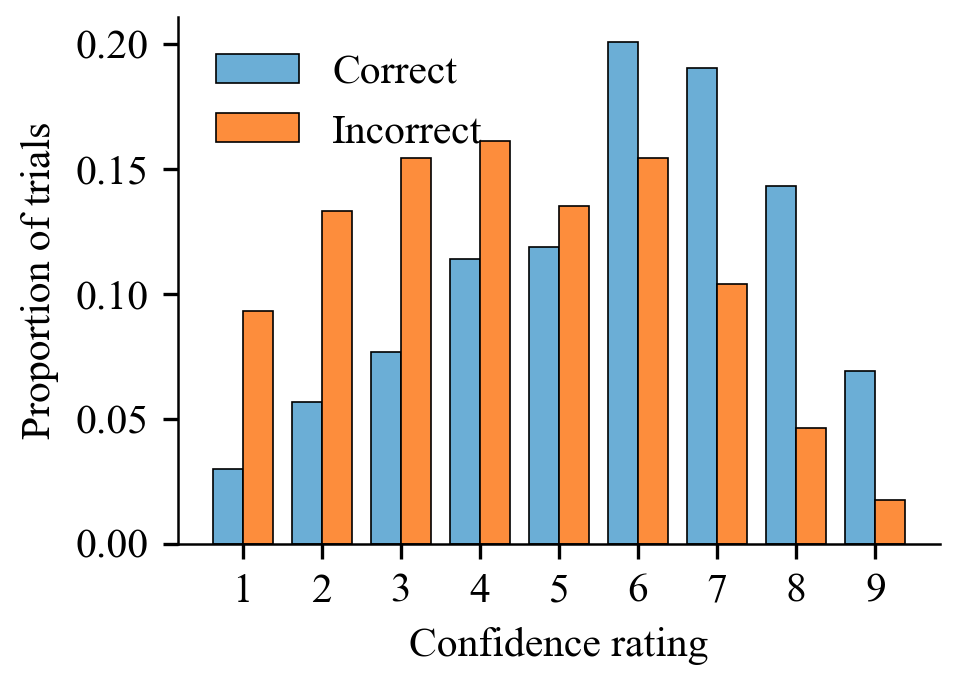
\includegraphics[width=0.55\textwidth]{figures/fig2.png}
\caption{Distribution of confidence ratings for correct and incorrect trials (all valid trials).}
\label{fig:conf}
\end{figure}

\subsection{RQ1 and RQ2: choice and accuracy}

Out-of-subject decoding of choice was above chance (mean AUC 0.526, SD 0.040; 18 of 24 participants above 0.5; permutation $p=0.010$), as was accuracy (mean AUC 0.535, SD 0.048; 18 of 24; $p=0.004$) (Table~\ref{tab:auc}, Fig.~\ref{fig:auc}). The permutation null had a mean of 0.501 and a 95th percentile of 0.517 for choice. Confidence (high versus low) behaved similarly (mean AUC 0.540, $p=0.006$). With Holm correction across these three primary tests the adjusted $p$-value was 0.012. Results were insensitive to the regularization strength and to shrinkage LDA (choice 0.526, accuracy 0.536), and the spatiotemporal variant gave 0.515 and 0.539. Within-participant cross-validation yielded 0.551 for choice and 0.541 for accuracy.

\begin{table}[ht]
\centering
\caption{Decoding performance (AUC)}
\label{tab:auc}
\small
\begin{tabular}{@{}lccc@{}}
\toprule
& \textbf{Choice} & \textbf{Accuracy} & \textbf{Confidence}\\
\midrule
LOSO, mean (SD) & 0.526 (0.040) & 0.535 (0.048) & 0.540 (0.065)\\
Permutation $p$ & 0.010 & 0.004 & 0.006\\
LOSO, pooled & 0.521 & 0.538 & 0.546\\
Shrinkage LDA & 0.526 & 0.536 & --\\
Within-participant & 0.551 & 0.541 & --\\
RT only & 0.508 & 0.615 & 0.688\\
RT-residualized & 0.526 & 0.503 & 0.512\\
RT-resid.\ $p$ & 0.006 & 0.415 & 0.216\\
\bottomrule
\end{tabular}
\end{table}

\begin{figure}[ht]
\centering
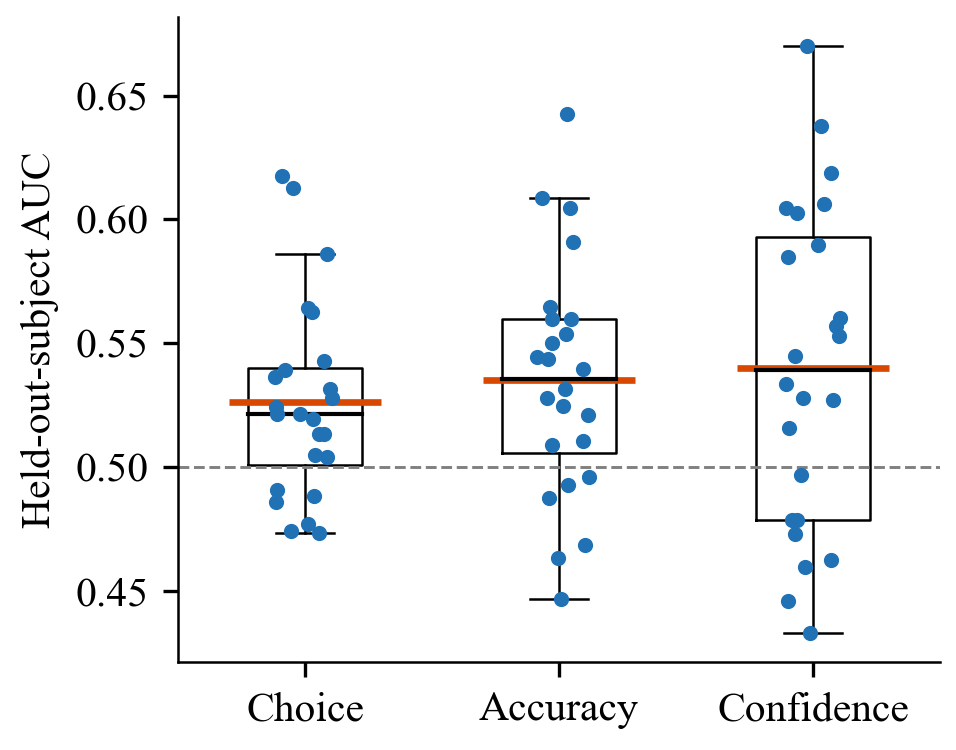
\includegraphics[width=0.55\textwidth]{figures/fig3.png}
\caption{Held-out-participant AUC for choice, accuracy, and confidence (high versus low). Dots are participants, boxes show quartiles, black lines the medians, and orange lines the means; the dashed line is chance.}
\label{fig:auc}
\end{figure}

Response time alone predicted accuracy (AUC 0.615) and confidence (0.688) better than the EEG did, but not choice (0.508). After removing the linear dependence of the EEG features on RT, choice decoding was unchanged (AUC 0.526, $p=0.006$), whereas accuracy decoding fell to chance (0.503, $p=0.415$) and so did confidence decoding (0.512, $p=0.216$). As a further control, the motion direction itself could be decoded from the same features (AUC 0.515), and the choice scores discriminated choice within each stimulus direction only weakly (AUC 0.516 and 0.519; permutation $p=0.043$ and $p=0.108$).

Stratifying by RT gave the same picture without a linear model. Within participant-specific RT terciles the mean AUC was 0.528 for choice ($p=0.006$, one-sided $t$-test), 0.517 for accuracy ($p=0.030$), and 0.495 for confidence ($p=0.619$). For choice the AUC was highest in the fastest tercile (0.551, versus 0.520 and 0.514), which is compatible with a larger motor or evidence contribution close to the response.

Participant-level AUCs varied considerably (Fig.~\ref{fig:auc}): choice 0.473 to 0.617, accuracy 0.447 to 0.643, and confidence 0.433 to 0.670. This spread is expected for small decoding effects in samples of 290 to 318 trials per participant and underlines why group-level inference was based on permutation of the whole procedure.

\subsection{Comparison decoders}

Table~\ref{tab:decoders} compares the primary decoder with the alternatives. No alternative was reliably better than logistic regression on mean amplitude: after Holm correction none exceeded it for any target, with or without the RT control. Shrinkage LDA and the linear SVM matched it (choice 0.525 and 0.527). The nonlinear models were not better: the RBF SVM, random forest, and perceptron reached 0.510, 0.511, and 0.517 for choice. The spatiotemporal variant gave the highest raw confidence AUC (0.563 with LDA), but the difference from the primary decoder was not significant and the value fell to 0.519 after RT control. Log-variance features produced AUCs significantly below 0.5 for accuracy and confidence (0.476 and 0.471); values below chance are not evidence of information and are a known artifact of cross-validation with participant-specific feature scales, so we do not interpret them. The conclusions therefore do not depend on the choice of classifier or on this feature type.

\begin{table}[ht]
\centering
\caption{Decoder comparison, raw/RT-residualized mean AUC}
\label{tab:decoders}
\small
\begin{tabular}{@{}lccc@{}}
\toprule
\textbf{Decoder} & \textbf{Choice} & \textbf{Accuracy} & \textbf{Confid.}\\
\midrule
Logistic (primary) & 0.527/.526 & 0.535/.503 & 0.541/.512\\
Shrinkage LDA & 0.525/.526 & 0.536/.505 & 0.541/.513\\
Linear SVM & 0.527/.526 & 0.535/.504 & 0.541/.512\\
RBF SVM & 0.510/.519 & 0.532/.503 & 0.550/.510\\
Random forest & 0.511/.511 & 0.533/.497 & 0.551/.511\\
Perceptron & 0.517/.514 & 0.522/.503 & 0.532/.502\\
Logistic, 4 bins & 0.515/.515 & 0.541/.514 & 0.560/.521\\
LDA, 4 bins & 0.514/.515 & 0.542/.512 & 0.563/.519\\
Logistic, log var. & 0.512/.506 & 0.476\textsuperscript{\dag}/.469 & 0.471\textsuperscript{\dag}/.477\\
Logistic, amp.\ + log var. & 0.530/.527 & 0.510\textsuperscript{\dag}/.481 & 0.506\textsuperscript{\dag}/.489\\
\bottomrule
\end{tabular}

\vspace{0.3em}
\begin{minipage}{0.92\textwidth}
\footnotesize \textsuperscript{\dag}\,Holm-corrected $p<0.05$ against the primary decoder (raw features). Entries are raw/RT-residualized mean held-out-participant AUC.
\end{minipage}
\end{table}

\subsection{Window sensitivity}

Fig.~\ref{fig:grid} shows mean AUC over a subset of the window grid. Values varied between 0.46 and 0.57 without a consistent optimum, and the selected window was not the best for any target; extreme cells should be read as chance variation across many comparisons, and no window was chosen from this analysis.

\begin{figure}[ht]
\centering
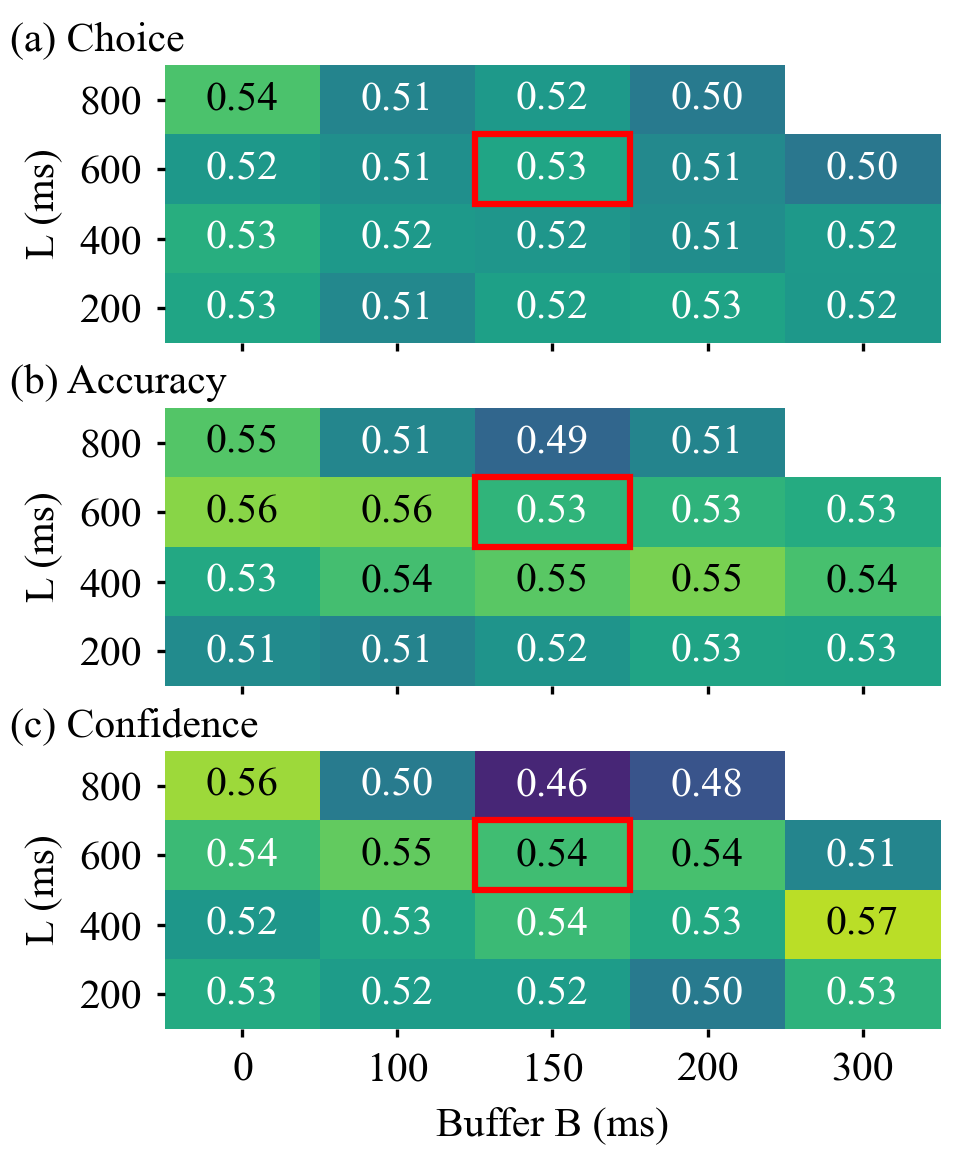
\includegraphics[width=\textwidth]{figures/fig4.png}
\caption{Sensitivity of mean held-out-participant AUC to window length $L$ and buffer $B$ for (a) choice, (b) accuracy, and (c) confidence. The red frame marks the pre-specified window. Blank cells have retention below 50\%.}
\label{fig:grid}
\end{figure}

\subsection{Time-resolved decoding}

Fig.~\ref{fig:time} shows the AUC in 100\,ms windows. Choice decoding fluctuated between 0.48 and 0.53 without a clear time course, and no window survived Holm correction. Accuracy decoding was significant after correction in three windows between 0.65 and 0.45\,s before the response (centers $-600$, $-550$, and $-400$\,ms; AUC 0.517 to 0.529), and none of these remained after RT residualization. Confidence decoding peaked at 0.541 in the window centered 200\,ms before the response but was not significant after correction. Choice AUC was highest in the window starting 150\,ms before the response (0.525, uncorrected $p=0.011$), which is compatible with a late motor-related contribution but is not significant after correction; the windows are short and the signals weak, so the time course is uninformative about the buffer.

\begin{figure}[ht]
\centering
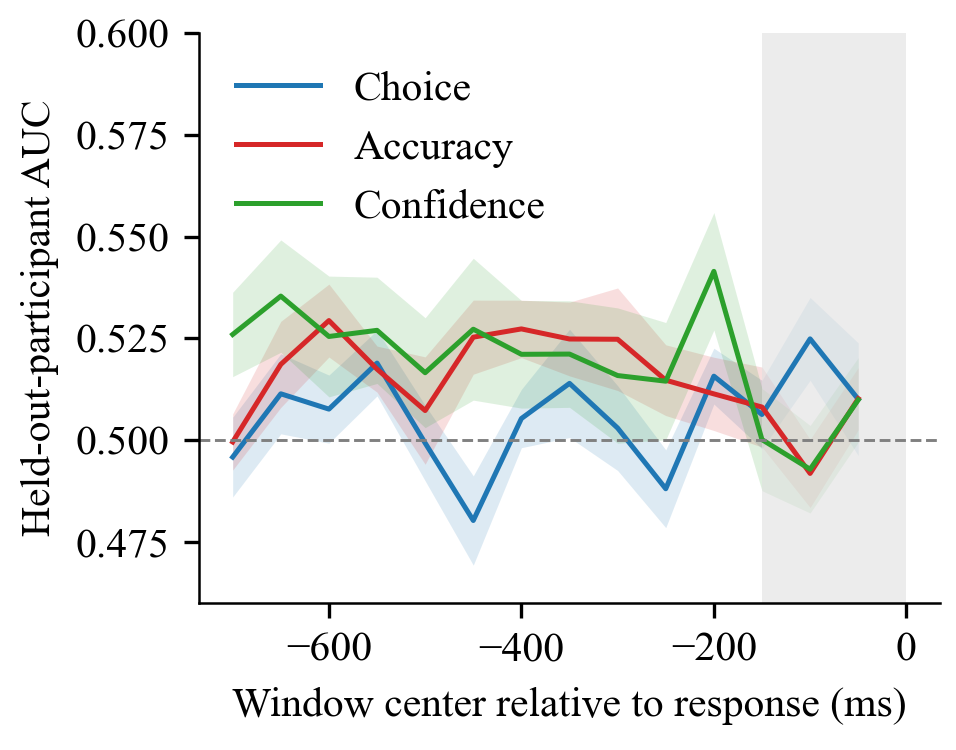
\includegraphics[width=\textwidth]{figures/fig5.png}
\caption{Time-resolved decoding with 100\,ms windows. Lines show the mean held-out-participant AUC against the window center, shaded areas the standard error across participants, and the gray band the buffer period excluded from the primary analysis.}
\label{fig:time}
\end{figure}

\subsection{RQ3: calibration}

Incorrect/high trials could not be distinguished from incorrect/low trials (pooled AUC 0.487, permutation $p=0.581$), nor reliably from correct/high trials (0.533, $p=0.104$) (Table~\ref{tab:calib}). The four-way classifier reached a balanced accuracy of 0.260 (chance 0.250) and a macro-averaged AUC of 0.516; no significance test was run for this analysis. In the two-stage analysis, incorrect/high trials had a slightly more correct-like accuracy-decoder score than incorrect/low trials (AUC 0.525, one-sided permutation $p=0.134$), which is the direction expected for an attenuated error signature but is not significant (Fig.~\ref{fig:violin}). Within participants, reported confidence correlated positively with the score on correct trials (mean Fisher $z=0.082$, $t(23)=3.52$, $p=0.002$) and weakly on incorrect trials (0.050, $p=0.087$); these correlations were not RT-controlled and should be read in light of the RT results above.

\begin{table}[ht]
\centering
\caption{Calibration contrasts (pooled AUC)}
\label{tab:calib}
\small
\begin{tabular}{@{}lrcc@{}}
\toprule
\textbf{Contrast} & \textbf{$n$} & \textbf{AUC} & \textbf{$p$}\\
\midrule
Incorr./high vs incorr./low & 853 & 0.487 & 0.581\\
Incorr./high vs corr./high & 1,866 & 0.533 & 0.104\\
Incorr./low vs corr./low & 1,455 & 0.516 & 0.218\\
\bottomrule
\end{tabular}
\end{table}

The calibration result depends little on how the confidence classes are defined (Table~\ref{tab:splits}). Among incorrect trials the high-versus-low AUC was 0.487 for ratings 1 to 3 versus 7 to 9, 0.537 for 1 to 2 versus 8 to 9, and 0.505 for 1 to 4 versus 6 to 9, with the strictest split borderline ($p=0.053$, 88 high-confidence errors). Among correct trials the contrast was above chance for all three splits and strongest for the strictest (0.552, $p=0.003$), but these correct-trial contrasts are not RT-controlled and, given the RT results, probably include response-speed information. The pattern, a larger separation among correct than among incorrect trials, is the opposite of what an attenuated pre-response error signature would predict if the EEG contained confidence information independent of accuracy.

\begin{table}[ht]
\centering
\caption{Confidence contrasts by definition of the classes (pooled AUC, $p$ in parentheses)}
\label{tab:splits}
\small
\begin{tabular}{@{}lcc@{}}
\toprule
\textbf{Split} & \textbf{Incorrect} & \textbf{Correct}\\
\midrule
Ratings 1--3 vs 7--9 & 0.487 (0.621) & 0.524 (0.040)\\
Ratings 1--2 vs 8--9 & 0.537 (0.053) & 0.552 (0.003)\\
Ratings 1--4 vs 6--9 & 0.505 (0.336) & 0.522 (0.023)\\
\bottomrule
\end{tabular}
\end{table}

\begin{figure}[ht]
\centering
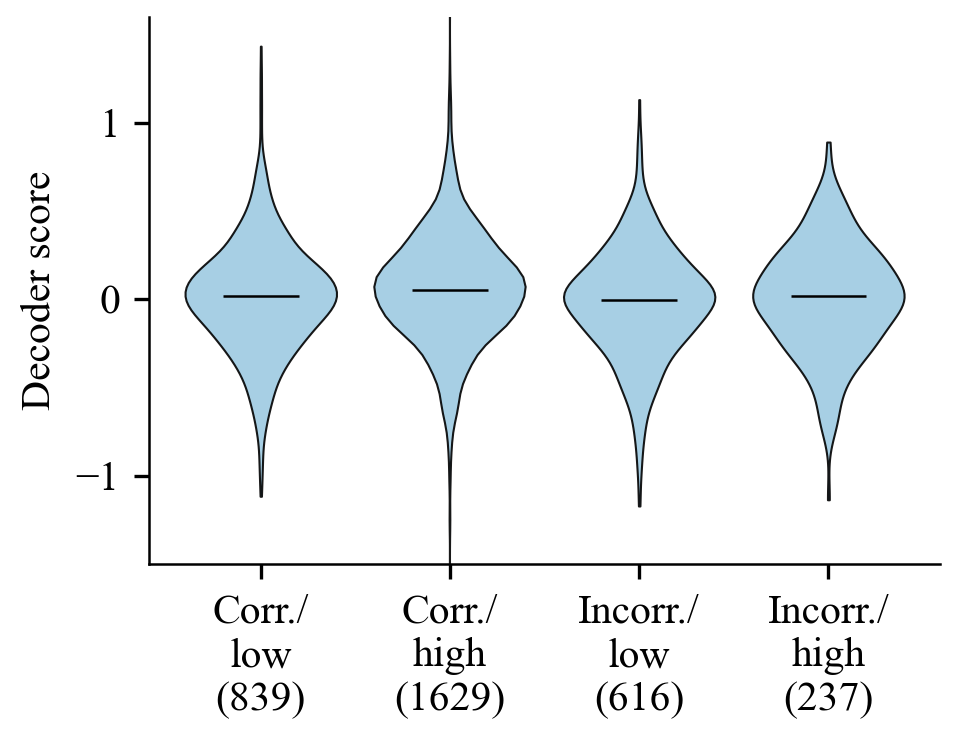
\includegraphics[width=0.55\textwidth]{figures/fig6.png}
\caption{Out-of-participant accuracy-decoder score by calibration cell (higher is more correct-like). Horizontal lines are medians; the vertical axis is truncated at the extremes.}
\label{fig:violin}
\end{figure}

\subsection{RQ4: sequential effects}

There were 5,332 consecutive trial pairs from 24 participants; the choice was repeated on 51.1\% and the motion direction on 49.1\% of pairs. The decoded neural confidence state did not predict choice repetition ($\beta=0.017$, SE 0.037, $p=0.648$), whereas reported confidence did ($\beta=0.143$, SE 0.048, $p=0.003$; Table~\ref{tab:gee}). With the stimulus-by-accuracy interaction included, the neural state remained null ($p=0.820$) and the reported-confidence effect was larger ($\beta=0.180$, $p<0.001$). Neither predictor was reliably related to the RT or the accuracy on trial $N{+}1$.

The covariates behaved as expected from the task structure. A repeated motion direction strongly raised the probability of repeating the choice ($\beta=1.153$, $p<0.001$), and with the interaction included the effect of a repeated direction was positive after a correct trial and negative after an error (interaction $\beta=4.304$), which mainly reflects that a correct response follows the stimulus. None of these covariate effects bears on the confidence question, and the interpretation of the confidence coefficients rests on their being estimated with these terms in the model.

\begin{table}[ht]
\centering
\caption{Predictors of trial $N{+}1$ behavior (GEE)}
\label{tab:gee}
\small
\begin{tabular}{@{}lcc@{}}
\toprule
\textbf{Outcome, predictor} & \textbf{$\beta$ (SE)} & \textbf{$p$}\\
\midrule
Repetition, neural & 0.017 (0.037) & 0.648\\
Repetition, reported & 0.143 (0.048) & 0.003\\
Log RT, neural & 0.000 (0.002) & 0.807\\
Log RT, reported & 0.004 (0.003) & 0.195\\
Accuracy, neural & 0.040 (0.031) & 0.188\\
Accuracy, reported & 0.018 (0.028) & 0.520\\
\bottomrule
\end{tabular}
\end{table}

%====================================================================
\section{Discussion}

\subsection{What the pre-response signal contains}

Pre-response EEG carried small but reliable information about the upcoming choice, and the effect survived the control for response time and the RT-tercile analysis. The within-participant estimate was higher than the out-of-participant estimate, which suggests that part of the signal is participant-specific and is lost when a single spatial filter is transferred across participants. We cannot attribute the choice signal to a particular source. Motor preparation is a plausible contributor despite the 150\,ms buffer, and the motion direction itself is weakly decodable (AUC 0.515), so the choice signal may reflect stimulus or evidence information as well as choice-specific activity. The result did not depend on the classifier: nonlinear models and alternative features did not improve on logistic regression (Table~\ref{tab:decoders}). The higher AUC in the fastest RT tercile is compatible with a stronger motor or evidence contribution near the response. Separating these sources would need a design that decouples stimulus, choice, and hand, or source-level analysis.

The accuracy and confidence effects are better explained by response speed. Both were predicted more strongly by RT than by the EEG, and both vanished after RT was regressed out of the features or after stratification by RT. A response-locked window places the EEG at different stimulus-relative times depending on RT, so EEG features can encode RT without any additional information about accuracy or confidence. This is consistent with a study that found no above-chance pre-response decoding of confidence \cite{r5}. It indicates that the earlier correlational finding for this dataset \cite{r2} does not translate into response-independent, out-of-participant prediction in our protocol. We do not compare AUC values with the original sliding-window analysis because the analysis differs in window, normalization, and validation, and we did not reproduce it.

\subsection{Calibration and sequential effects}

For calibration, we found no evidence that high-confidence errors are neurally distinguishable from low-confidence errors before the response. The direction of the two-stage effect matched the overconfidence hypothesis, but its size was small and not significant, so the data neither support nor exclude an attenuated pre-response error signature. The existing evidence for such signatures concerns post-response components \cite{r3,r4}, which our window by design excludes, and a study of confidence in a different time window found partly distinct pre- and post-response markers \cite{r18}. The sensitivity analysis showed a larger separation among correct than among incorrect trials, which fits the interpretation that the decoder tracks response speed more than confidence-specific error signals.

For sequential effects, reported confidence predicted choice repetition, in line with confidence-weighted choice history \cite{r20}, whereas the decoded neural state did not. Because the neural proxy is itself weak (AUC about 0.54) and largely reflects RT, this null result is expected and is not evidence against a neural account. A fair test would use a stronger confidence readout, for example a post-response component, and a model-based estimate of the decision bound \cite{r22}.

\subsection{Effect sizes and reporting}

The design also determines what effect sizes could have been detected. With 24 participants the permutation null for the mean AUC had a standard deviation of about 0.010 to 0.012 and a 95th percentile of 0.517 to 0.519, so mean AUCs of about 0.52 or higher were detectable, whereas the individual participant AUCs spread over roughly 0.43 to 0.67. An AUC of 0.52 corresponds to a very small shift in the score distributions, and decisions based on a single trial would be barely better than guessing. The practical consequence is that these pre-response features cannot be used to flag an individual overconfident response in this paradigm.

The results also bear on how pre-response decoding studies should be reported. First, any target correlated with response time needs an RT-controlled analysis, because a response-locked window makes EEG features a proxy for RT. Second, class balance and subject diversity of rare cells, such as high-confidence errors, should be shown before the main analysis. Third, normalization and model fitting must be organized so that no information from the held-out participant's labels is used. Finally, weak or null results should be reported together with their permutation null so that readers can judge the effect size.

%====================================================================
\section{Limitations and Threats to Validity}

\subsection{Internal validity}

All relationships are predictive and correlational, and no causal role of the EEG activity is implied. The RT control removes only linear dependence, and the stimulus-direction control is partial, so residual contamination by response speed or stimulus information cannot be excluded for the choice result. The in-scanner EEG may retain residual gradient or ballistocardiogram artifacts despite the correction applied by the dataset authors, and artifacts with a systematic relation to the heartbeat could in principle covary with RT.

\subsection{Construct validity}

Confidence is operationalized by a coarse split of a 9-point rating, and overconfidence by a single high-confidence error, which ignores the metacognitive sensitivity of each participant \cite{r19}. The decision bound is not estimated, since no diffusion model was fitted, so RT and accuracy on the next trial are only proxies. The decoded neural confidence state is weak and probably contaminated by RT, which limits its use as a measure of trial-wise confidence.

\subsection{External validity}

The window rule excluded the fastest 17.4\% of trials, which were also the more accurate and confident ones, so the results apply to slower trials. Only 53 channels common to all participants were used. The sample consists of 24 participants performing one motion task with a calibrated difficulty, and the findings may not transfer to other tasks, difficulty levels, or recording settings.

\subsection{Statistical conclusion validity}

The window grid contains many comparisons, so its extreme cells are optimistic, and the time-resolved analysis was added after the primary analysis. The four-way RQ3 classifier was not tested for significance and the incorrect/high class remains small. Several analysis choices, including $C$, the LOSO scheme, and the RT control, were fixed by the analysts without external review. The sequential models assume an exchangeable within-participant correlation and include only a few covariates. The comparison decoders used fixed, untuned hyperparameters, and no deep convolutional network was included, so a better-tuned or end-to-end model cannot be excluded as able to extract more information.

%====================================================================
\section{Conclusion and Future Work}

In 24 participants, EEG recorded 600 to 150\,ms before the response predicted the upcoming choice with a small effect (AUC 0.526), and also accuracy and confidence, but the accuracy and confidence effects are accounted for by response time. High-confidence errors were not separable from low-confidence errors, and the decoded neural confidence did not predict next-trial behavior. Five alternative classifiers and three feature sets did not do better. The study provides a leakage-controlled protocol, an explicit response-time control, and the class-balance numbers needed to plan better-powered tests. Future work should (i) match trials on RT and stimulus direction, (ii) fit sequential-sampling models to estimate decision bounds, (iii) combine pre- and post-response windows, (iv) use time-resolved, end-to-end, and EEG-fMRI-informed decoders, and (v) test in larger samples whether pre-response EEG adds predictive information beyond behavior.

\section*{Conflicts of Interest}
The authors declare no conflict of interest.

\section*{Data and Code Availability}
The EEG-fMRI data are publicly available at OpenNeuro (ds002739, DOI 10.18112/openneuro.\allowbreak ds002739.v1.0.0). This study analyzed these de-identified data and collected no new data. [AUTHORS TO CONFIRM whether your institution requires an ethics statement for secondary analysis, and where the analysis code will be deposited.]

\section*{Acknowledgments}
The EEG-fMRI data were collected and shared by S.\ Gherman and M.\ G.\ Philiastides (OpenNeuro ds002739, CC0). Generative AI (Claude, Anthropic) was used to write and run the analysis code and to draft the text; the authors are responsible for reviewing and approving all content.

%====================================================================
\begin{thebibliography}{99}
\bibitem{r1} S. Gherman and M. G. Philiastides, ``Simultaneous EEG-fMRI -- Confidence in perceptual decisions,'' \textit{OpenNeuro}, ds002739, Version 1.0.0, DOI: 10.18112/openneuro.ds002739.v1.0.0, 2020.
\bibitem{r2} S. Gherman and M. G. Philiastides, ``Human VMPFC encodes early signatures of confidence in perceptual decisions,'' \textit{eLife}, vol.~7, Art.~no.~e38293, 2018.
\bibitem{r3} A. Boldt and N. Yeung, ``Shared neural markers of decision confidence and error detection,'' \textit{Journal of Neuroscience}, vol.~35, no.~8, pp.~3478--3484, 2015.
\bibitem{r4} K. Desender, K. R. Ridderinkhof, and P. R. Murphy, ``Understanding neural signals of post-decisional performance monitoring: An integrative review,'' \textit{eLife}, vol.~10, Art.~no.~e67556, 2021.
\bibitem{r5} K. Desender, P. Murphy, A. Boldt, T. Verguts, and N. Yeung, ``A postdecisional neural marker of confidence predicts information-seeking in decision-making,'' \textit{Journal of Neuroscience}, vol.~39, no.~17, pp.~3309--3319, 2019.
\bibitem{r6} R. G. O'Connell, P. M. Dockree, and S. P. Kelly, ``A supramodal accumulation-to-bound signal that determines perceptual decisions in humans,'' \textit{Nature Neuroscience}, vol.~15, no.~12, pp.~1729--1735, 2012.
\bibitem{r7} S. P. Kelly and R. G. O'Connell, ``Internal and external influences on the rate of sensory evidence accumulation in the human brain,'' \textit{Journal of Neuroscience}, vol.~33, no.~50, pp.~19434--19441, 2013.
\bibitem{r8} J. Herding, S. Ludwig, A. von Lautz, B. Spitzer, and F. Blankenburg, ``Centro-parietal EEG potentials index subjective evidence and confidence during perceptual decision making,'' \textit{NeuroImage}, vol.~201, Art.~no.~116011, 2019.
\bibitem{r9} S. Gluth, J. Rieskamp, and C. B\"uchel, ``Classic EEG motor potentials track the emergence of value-based decisions,'' \textit{NeuroImage}, vol.~79, pp.~394--403, 2013.
\bibitem{r10} M. G. Philiastides, R. Ratcliff, and P. Sajda, ``Neural representation of task difficulty and decision making during perceptual categorization: A timing diagram,'' \textit{Journal of Neuroscience}, vol.~26, no.~35, pp.~8965--8975, 2006.
\bibitem{r11} R. Ratcliff, M. G. Philiastides, and P. Sajda, ``Quality of evidence for perceptual decision making is indexed by trial-to-trial variability of the EEG,'' \textit{Proceedings of the National Academy of Sciences}, vol.~106, no.~16, pp.~6539--6544, 2009.
\bibitem{r12} P. Sajda, M. Philiastides, and L. Parra, ``Single-trial analysis of neuroimaging data: Inferring neural networks underlying perceptual decision-making in the human brain,'' \textit{IEEE Reviews in Biomedical Engineering}, vol.~2, pp.~97--109, 2009.
\bibitem{r13} C. S. Soon, M. Brass, H.-J. Heinze, and J.-D. Haynes, ``Unconscious determinants of free decisions in the human brain,'' \textit{Nature Neuroscience}, vol.~11, no.~5, pp.~543--545, 2008.
\bibitem{r14} S. Bode, A. H. He, C. S. Soon, R. Trampel, R. Turner, and J.-D. Haynes, ``Tracking the unconscious generation of free decisions using ultra-high field fMRI,'' \textit{PLoS ONE}, vol.~6, no.~6, Art.~no.~e21612, 2011.
\bibitem{r15} M. K. van Vugt, M. A. Beulen, and N. A. Taatgen, ``Relation between centro-parietal positivity and diffusion model parameters in both perceptual and memory-based decision making,'' \textit{Brain Research}, vol.~1715, pp.~1--12, 2019.
\bibitem{r16} L. Charles, F. Van Opstal, S. Marti, and S. Dehaene, ``Distinct brain mechanisms for conscious versus subliminal error detection,'' \textit{NeuroImage}, vol.~73, pp.~80--94, 2013.
\bibitem{r17} L. Charles, J.-R. King, and S. Dehaene, ``Decoding the dynamics of action, intention, and error detection for conscious and subliminal stimuli,'' \textit{Journal of Neuroscience}, vol.~34, no.~4, pp.~1158--1170, 2014.
\bibitem{r18} M. Rausch, M. Zehetleitner, M. Steinhauser, and M. E. Maier, ``Cognitive modelling reveals distinct electrophysiological markers of decision confidence and error monitoring,'' \textit{NeuroImage}, vol.~218, Art.~no.~116963, 2020.
\bibitem{r19} S. M. Fleming and H. C. Lau, ``How to measure metacognition,'' \textit{Frontiers in Human Neuroscience}, vol.~8, Art.~no.~443, 2014.
\bibitem{r20} A. Braun, A. E. Urai, and T. H. Donner, ``Adaptive history biases result from confidence-weighted accumulation of past choices,'' \textit{Journal of Neuroscience}, vol.~38, no.~10, pp.~2418--2429, 2018.
\bibitem{r21} A. E. Urai, A. Braun, and T. H. Donner, ``Pupil-linked arousal is driven by decision uncertainty and alters serial choice bias,'' \textit{Nature Communications}, vol.~8, no.~1, Art.~no.~14637, 2017.
\bibitem{r22} K. Desender, A. Boldt, T. Verguts, and T. H. Donner, ``Confidence predicts speed-accuracy tradeoff for subsequent decisions,'' \textit{eLife}, vol.~8, Art.~no.~e43499, 2019.
\bibitem{r23} E. Combrisson and K. Jerbi, ``Exceeding chance level by chance: the caveat of theoretical chance levels in brain signal classification and statistical assessment of decoding accuracy,'' \textit{Journal of Neuroscience Methods}, vol.~250, pp.~126--136, 2015.
\bibitem{r24} B. Blankertz, S. Lemm, M. Treder, S. Haufe, and K.-R. M\"uller, ``Single-trial analysis and classification of ERP components -- A tutorial,'' \textit{NeuroImage}, vol.~56, no.~2, pp.~814--825, 2011.
\bibitem{r25} O. Ledoit and M. Wolf, ``A well-conditioned estimator for large-dimensional covariance matrices,'' \textit{Journal of Multivariate Analysis}, vol.~88, no.~2, pp.~365--411, 2004.
\bibitem{r26} M. Ojala and G. C. Garriga, ``Permutation tests for studying classifier performance,'' in \textit{Proc.\ IEEE International Conference on Data Mining}, pp.~908--913, 2009.
\bibitem{r27} K.-Y. Liang and S. L. Zeger, ``Longitudinal data analysis using generalized linear models,'' \textit{Biometrika}, vol.~73, no.~1, pp.~13--22, 1986.
\end{thebibliography}

\end{document}
